% !TeX spellcheck = en_CA
\documentclass[11pt,oneside]{book}
\usepackage{amsmath}
\usepackage{amssymb}
\usepackage{makeidx}
\usepackage[english]{babel}
\usepackage[utf8]{inputenc}
\usepackage[margin=2.5cm,left=3cm]{geometry}
%\usepackage{pdfcomment}
\usepackage{algorithm}
\usepackage[noend]{algpseudocode}
\usepackage[nottoc]{tocbibind}
\usepackage{xcolor}
\usepackage[pdftex,colorlinks=true,linkcolor=blue,citecolor=red]{hyperref}
\usepackage{datetime}
\usepackage{lipsum}


%% Automaticky generovane zkratky
\usepackage[xindy]{glossaries}
\makeglossaries
% Specialni znaky


% Obycejne zkratky
% \newacronym{}{, first={ ()}
\newacronym{FIFO}{FIFO}{first-in first-out} 


% Symboly


%\addto\captionsenglish{\renewcommand{\figurename}{Fig.}}
\newcommand{\figref}[1]{\figurename~\ref{#1}}
\newcommand{\tabref}[1]{Table \ref{#1}}
\newcommand{\secref}[1]{Section \ref{#1}}



% Document metadata
\author{Ing. Name Surname}
\title{Very Long Name of Disertation Thesis Dealing With Some Science}
	

\begin{document}

\frontmatter
\maketitle


\chapter*{Abstract}
\addcontentsline{toc}{chapter}{Abstract}

% Random text
\lipsum[0-4]


\vspace{3mm}
\noindent
\textbf{Keywords:}
Optical burst switching, loss-less, operational research, column generation, simulations.







\newpage
\chapter*{Acknowledgements}
\addcontentsline{toc}{chapter}{Acknowledgements}

\lipsum[2-4]
\tableofcontents


\mainmatter
\chapter{Introduction} \label{sec:introdution}
\lipsum 

\begin{figure}[h]
	\centering
	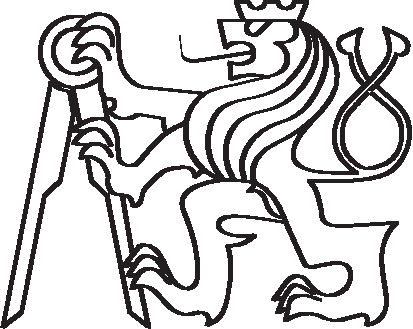
\includegraphics[width=0.5\linewidth]{images/LogoCVUT.pdf}
	\caption{Logo CVUT. }
	\label{fig:cvut}
\end{figure}

% ---------------------------------------------------------------------------------------------------------------
% ---------------------------------------------------------------------------------------------------------------
% ---------------------------------------------------------------------------------------------------------------
\chapter{Disertation thesis targets} 
\lipsum 



% ---------------------------------------------------------------------------------------------------------------
% ---------------------------------------------------------------------------------------------------------------
% ---------------------------------------------------------------------------------------------------------------
\chapter{Article 1} 
\lipsum 
% First time use of an acronym
\gls{FIFO}

This is reference to CTU logo: \figref{fig:cvut}

This is reference to a chapter: \secref{sec:introdution}

This is reference to a table: \tabref{tab:example}




% ---------------------------------------------------------------------------------------------------------------
% ---------------------------------------------------------------------------------------------------------------
% ---------------------------------------------------------------------------------------------------------------
\chapter{Article 2} 
\lipsum 

% Citation from BIB file
\cite{rfc6462,rfc6463,rfc6468,rfc6470,rfc6471,rfc6475}

\begin{table*}
	\scriptsize
	\centering
	\caption{An example of traffic pattern used for XXX topology.}
	\begin{tabular}{c|rrrrrrrrrrrr}
		{} &       0  &       1  &       2  &       3  &       4  &       5  &       6  &       7  &       8  &       9  &       10 &       11 \\
		\hline
		0  &      X &   158.32 &  7774.43 &  7738.39 &  7512.69 &  2186.25 &  1722.48 &  4284.82 &  5330.93 &  5865.15 &  9152.69 &  1485.00 \\
		1  &  2818.68 &      X &  3621.17 &  5917.80 &  5524.19 &  9891.76 &  1524.97 &   880.77 &  8582.06 &  4733.80 &  5291.90 &  5689.95 \\
		2  &  9699.68 &  8482.77 &      X &  5269.06 &  3397.06 &  1425.16 &   113.21 &  2415.42 &  2360.39 &  9517.65 &  7743.05 &  3221.60 \\
		3  &  1138.69 &  3018.70 &  4620.40 &      X &  4864.32 &  9299.88 &  7181.59 &  3626.95 &  5388.13 &  4414.69 &  9065.83 &  6194.78 \\
		4  &  7627.29 &  3018.82 &  9128.96 &  8487.32 &      X &    79.14 &   145.06 &  3931.23 &  8659.49 &  3802.32 &  4648.42 &  4480.67 \\
		5  &  2296.11 &  2774.38 &  1457.50 &  1976.43 &  2054.90 &      X &  3316.93 &  7235.76 &  8242.63 &  7655.13 &  4469.84 &  7302.30 \\
		6  &  9003.56 &   575.16 &  8883.98 &  9673.00 &  4547.04 &   748.82 &      X &  8685.67 &  7323.91 &     5.29 &  9681.16 &   465.38 \\
		7  &  7097.11 &  1981.23 &  4030.56 &  2286.47 &  7551.73 &   852.78 &  7735.45 &      X &    43.08 &  4579.22 &  7265.16 &  3516.30 \\
		8  &  9949.75 &  2235.61 &  1203.04 &  5968.25 &   120.27 &  7473.08 &  5113.32 &  1956.49 &      X &   511.18 &  5738.25 &  9124.52 \\
		9  &  1732.57 &  7462.56 &  4159.81 &   909.00 &  3100.43 &  6559.28 &  7596.25 &  9376.22 &  2019.94 &      X &  5770.77 &  8697.44 \\
		10 &  5310.71 &  8055.50 &  4693.06 &  2780.88 &  5233.34 &  9709.97 &  9924.73 &  8123.84 &  9588.17 &  4978.55 &      X &   215.05 \\
		11 &  1488.95 &  7047.40 &  7963.36 &  3767.27 &  4908.68 &  2071.56 &  4511.59 &  9631.70 &  4085.00 &  4390.31 &  2959.40 &      X \\
	\end{tabular}
	\label{tab:example}
\end{table*}


% ---------------------------------------------------------------------------------------------------------------
% ---------------------------------------------------------------------------------------------------------------
% ---------------------------------------------------------------------------------------------------------------
\chapter{Article 3} 
\lipsum 
% Second time use of an acronym
\glspl{FIFO}




% ---------------------------------------------------------------------------------------------------------------
% ---------------------------------------------------------------------------------------------------------------
% ---------------------------------------------------------------------------------------------------------------
\chapter{Conclusion}
\section{Summary of thesis} \lipsum
\section{Fulfilments of targets} \lipsum
\section{Further extensibility and recommendations} \lipsum



\appendix
\chapter{Extra 1} \lipsum
\chapter{Extra 2} \lipsum


\backmatter
\bibliographystyle{IEEEtran} %The style you want to use for references.
\bibliography{literature}


\end{document}
